%
% 5_Anwendungen.tex -- Eine kurze Vorstellung der Anwendungsgebiete der Methode der finiten Elemente
%
% (c) 2024 Flurin Brechbühler, OST - Ostschweizer Fachhochschule Rapperswil
%
% !TEX root = ../../buch.tex
% !TEX encoding = UTF-8
%
\section{Anwendungen\label{fem:section:anwendungen}}
\kopfrechts{Anwendungen}

Die Methode der finiten Elemente findet überall wo Differenzialgleichungen vorkommen Verwendung.
Einige Beispiele dazu sind:
\begin{itemize}
    \item [\textbf{Strukturelle Simulationen,}] um die Beanspruchung von komplexen Bauten wie Brücken oder mechanischen Bauteilen wie Zahnprothesen vorherzusagen.
    \item [\textbf{Thermische Simulationen,}] die Auskunft darüber geben, wie sich zum Beispiel die Wärme in einer Bremse oder einem Wärmetauscher verteilt.
    \item [\textbf{Aero- und hydrodynamische Simulationen,}] mit denen zum Beispiel der Luftstrom über einen Flügel oder der Wasserstrom über eine Turbine simuliert werden kann.
    \item [\textbf{Elektromagnetische Simulationen,}] um zum Beispiel das Abstrahlverhalten von Antenne vorherzusagen.
\end{itemize}

Oft wird für jedes Teilgebiet eine separate spezialisierte Softwaresuite verwendet.
Wer jedoch mal die Welt der durch die FEM ermöglichten Simulationen erkunden möchte, kann seine ersten Schritte sehr wohl auch mit etwas weiter verbreiteter Software tun: 
Die PDE-Toolbox von Matlab bietet eine Umgebung, mit der durch sehr wenig Aufwand beeindruckende Ergebnisse erzielt werden können.
Man kann so zum Beispiel eine .STL-Datei (also ein 3D-Modell) eines Balkens laden und die Problemdomäne von Matlab diskretisieren, beziehungsweise ein dazugehöriges Mesh generieren lassen. 
%
% balken_mesh.tex
%
% (c) 2024 Flurin Brechbühler
%
\begin{figure}
    \centering
    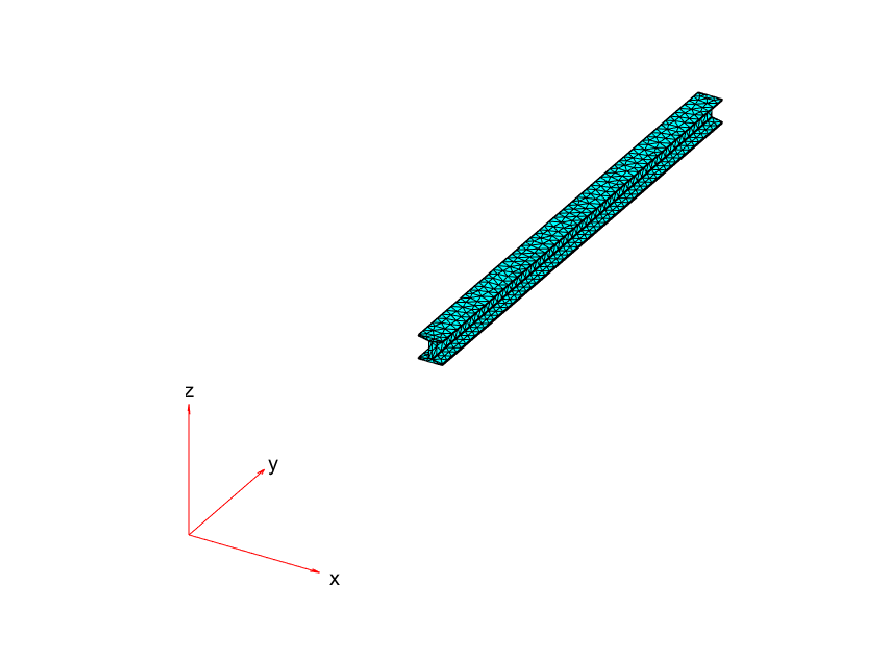
\includegraphics[width=\textwidth]{papers/fem/images/balken_mesh.pdf}
    \caption{Das in dreieckige Elemente unterteilte 3D-Modell des Balkens.}
    \label{fem:anw:mesh}
    \end{figure}
    
Das resultierende Mesh ist in Abb. \ref{fem:anw:mesh} ersichtlich.
Nun können durch einige wenige Befehle die Randbedingungen festgelegt und anschliessend die Simulation gestartet werden.
%
% balken_resultat.tex
%
% (c) 2024 Flurin Brechbühler
%
\begin{figure}
    \centering
    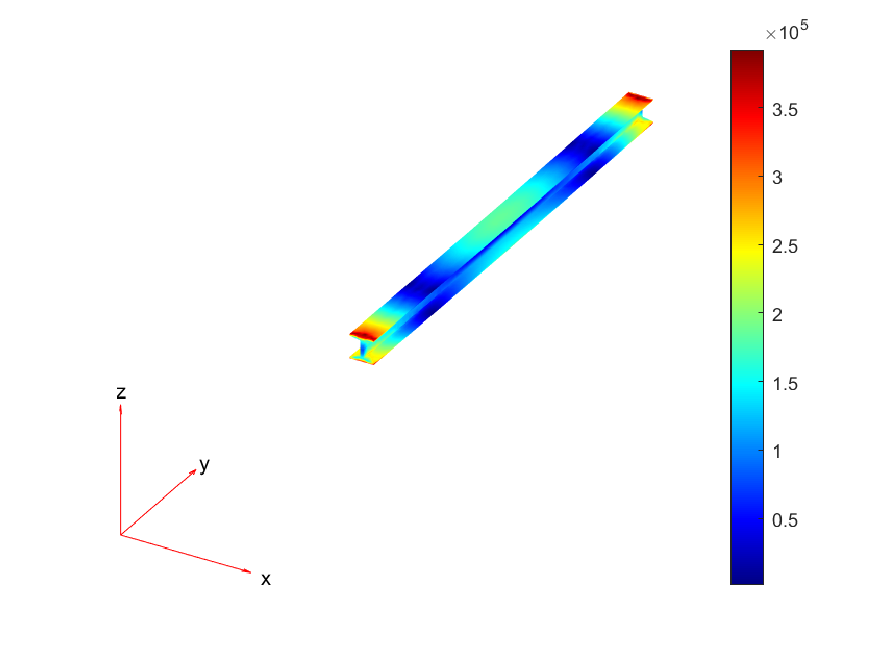
\includegraphics[width=\textwidth]{papers/fem/images/balken_resultat.pdf}
    \caption{Das in Matlab erhaltene Resultat der strukturellen Simulation.}
    \label{fem:anw:resultat}
    \end{figure}
    
Es resultiert das in Abb. \ref{fem:anw:resultat} abgebildete Resultat der Simulation, in dem durch den Farbgradienten die Belastung, sowie (überhöht dargestellt) die zu erwartende Deformation zu erkennen ist.
Die FEM kann also auch für dieses in Kapitel \ref{chapter:balken} beschriebene Problem 4. Ordnung sehr gut eingesetzt werden.